% ============================================
%  Article Class (This is a LaTeX2e document)  
% ============================================
\documentclass[12pt]{scrartcl}

\usepackage[french]{babel}
\usepackage[utf8]{inputenc}

\usepackage{enumitem}
\usepackage[round]{natbib}
\usepackage{color}

\newcommand\reft[3][]{#2~\ref{#3}#1}
\newcommand\refp[3][]{(#2~\ref{#3}#1)}
\newcommand\refsect[1]{\reft{Section}{#1}}
\newcommand\refsecp[1]{\refp{Sec.}{#1}}
\newcommand\reftabt[1]{\reft{Table}{#1}}
\newcommand\reftabp[1]{\refp{Tab.}{#1}}

% ============
%  Algorithms
% ============
\usepackage{algorithm2e}
\SetKwProg{Fn}{Function}{}{}
\newcommand\refalgt[1]{\reft{Algorithm}{#1}}
\newcommand\refalgp[1]{\refp{Alg.}{#1}}

% ======
%  Math
% ======
\usepackage{amsmath}
\usepackage{amsthm}
\newtheorem{thm}{Theorem}[section]
\newtheorem{cor}[thm]{Corollary}
\newtheorem{lem}[thm]{Lemma}
\newtheorem{prop}[thm]{Proposition}
\newtheorem{property}[thm]{Property}
\theoremstyle{definition}
\newtheorem{defn}[thm]{Definition}
\newtheorem{assum}[thm]{Assumption}
\theoremstyle{remark}
\newtheorem{rem}[thm]{Remarque}
\numberwithin{equation}{section}
\usepackage{amssymb}
\newcommand{\prob}[1]{\mathbb{P}\left(#1\right)}

% ============================
%  Figures and relative paths
% ============================
\usepackage{graphicx}
\graphicspath{{figures/}}
\usepackage{import}
\makeatletter
  \def\relativepath{\import@path}
\makeatother
\newcommand\reffigt[2][]{\reft[#1]{Figure}{#2}}
\newcommand\reffigp[2][]{\refp[#1]{Fig.}{#2}}

% ==========
%  Document
% ==========
\begin{document}

\title{Bibliographie RBA pour les plantes}%
\author{S. Fischer - Biosys - MAIAGE}%
\date{\today}%

\maketitle

\newpage

\tableofcontents

\newpage

\section{Les concepts de bases}

\subsection{FBA}

\paragraph{Formulation} Je reprends la façon dont c'est cité dans l'intro de \citet{goelzer_cell_2011}. Le formalisme des FBA est très simple: on se donne un certain nombre de métabolites et de réactions, une matrice de stoechiométrie $S$ qui représente les réactions et des flux $\nu$ pour chaque réaction. Le problème d'optimisation est juste donné par
\[
\left\lbrace
\begin{array}{l}
  \textrm{Maximiser } c^T\nu \\
  \textrm{sous les contraintes } S\nu=b, \alpha_i \leq \nu_i \leq \beta_i
\end{array}
\right.
\]
$b$ est nul s'il n'y a pas de flux entrant.

\begin{rem}
Dans le domaine, on identifie volontiers une réaction par l'enzyme qui la catalyse. Pour l'instant je ne sais pas trop ce qui se passe si une enzyme catalyse deux réactions différentes. En tout cas il ne faut pas s'étonner si les dimensions de $S$ sont données en fonction du nombre d'enzymes et pas du nombre de réactions.
\end{rem}

\begin{rem}
Implicitement, il semble que le système soit réécrit en tenant compte des sens de réactions et en forçant $\nu \geq 0$ \citep{savinell_network_1992}!!! Ça rajoute pas mal de contraintes.
\end{rem}

\begin{rem}
La matrice de stoechiométrie peut être simplifiée en agrégeant des réactions \citep{varma_metabolic_1993}.
\end{rem}

\begin{rem}
La formulation duale du problème est utilisée pour juger l'importance de chaque métabolite à réaliser un objectif précis. Ça a été formalisé avec les idées de \textit{shadow price} et \textit{reduced costs} \citep{savinell_network_1992} et  \textit{scaled shadow price} \citep{varma_metabolic_1993-1}.
\end{rem}

\paragraph{Problèmes} (1) on est obligé de minorer/majorer certaines valeurs de $\nu$ pour borner l'espace des solutions, (2) le vecteur $c$ est fixé \textit{a priori}. Il donne les flux nécessaires à soutenir un certain taux de croissance (notamment en contrôlant les flux des métabolites finaux), mais la composition dépend en réalité du taux de croissance.

\paragraph{Interprétation mathématique} La première contrainte est un simple système linéaire. Si $b=0$, $\nu$ vit dans le noyau de $S$ (typiquement un espace vectoriel non borné de type $\mathbb{R}^n$). Si $b$ est non nul, $\nu$ vit dans un espace affine $\nu_0 + \mathrm{Ker}S$ (sensiblement la même chose). Une base naturelle du noyau est donné par les cycles minimaux du système. Imposer $b$ ne diminue pas la dimension de l'espace des solutions...

$c^T\nu$ est un produit scalaire. Sur une sphère unité du noyau, il est maximal dans la direction de la projection de $c$ sur l'espace des solutions. Mais vu que cet espace n'est pas borné, il est évident qu'il n'y a pas de solution (sauf si $c$ est orthogonal à l'espace des solutions...). On peut même ajouter que dès qu'une des dimensions de l'espace (non orthogonale à $c$) n'est pas bornée, il n'y a pas de solution. Il faut donc autant de contraintes (indépendantes) sur $\nu$ que de dimensions au noyau de $S$.

En imposant des bornes sur chaque composante de $\nu$ on découpe le s.e.v de façon à le borner en un espace convexe. Le produit scalaire est forcément maximal sur un bord de l'espace découpé. Vu que le bord est linéaire par morceau et que $c^T\nu$ est proportionnel à la projection de $\nu$ sur $c$, on peut se convaincre que c'est maximal sur un sommet (sauf si une arête/face est ortogonale à $c$, blablabla - rien de nouveau pour de l'optimisation linéaire en espace convexe, c'est juste pour donner une image). Vu que le sommet est donné par le découpage des $\alpha$ et $\beta$, il y a un risque quee ce découpage détermine la solution finale. Normalement, si on est obligés de définir des $\beta_i$, c'est qu'ils devraient intervenir dans la solution. Par contre difficile d'évaluer en grande dimension à quel point l'orientation de $c$ peut faire basculer la solution d'un sommet à l'autre ou à quel point ce basculement peut avoir des effets catastrophiques?

Certains auteurs n'imposent pas de bornes sur $\nu$ \citep{varma_metabolic_1993, varma_metabolic_1993-1} et se donnent un certain $b$. Ici intervient la contrainte cachée $\nu \geq 0$ et la décomposition des réactions bidirectionnelles en réactions unidirectionnelles. Cela supprime de l'espace des solutions tous les cycles infaisables d'un point de vue thermodynamique et limite la dégénrescence des solutions aux cycles faisables. La solution est unique ssi le noyau de $A$ ne s'intersecte pas avec le sous-espace $\nu \geq 0$. 

\begin{rem}
La dimension la plus grand de $S$ est visiblement le nombre de réactions, pas le nombre de métabolites. Il faudrait réfléchir au rang (plein?) de $S$ (et du coup à la dimension du noyau).
\end{rem}


\paragraph{Variantes?} Le problème est clairement formulé comme \citet{goelzer_cell_2011} dans \citet{fell_fat_1986} (parfois considéré comme l'article fondateur). Pourtant dans \citet{varma_metabolic_1993-1, varma_stoichiometric_1994}, la formulation de la fonction objectif est différente, l'objectif est exprimé en fonction des métabolites. Dans tous les cas, il semble qu'on identifie un métabolisme à son flux de sortie, mais comment on fait pour construire $c$ quand plusieurs réactions produisent un élément (comme l'ATP ou le NADH)? Le seul article qui explique clairement sa procédure est \citet{savinell_network_1992}, où les coûts sont répartis uniformément. Ceci étant dit, dans cet article on ne cherche pas à maximiser la croissance de biomasse, mais à minimiser le coût de la croissance!

Le choix de la contrainte qui permet de fixer la solution n'est pas toujours la même. Dans \citet{savinell_network_1992, varma_metabolic_1993, varma_metabolic_1993-1} $A$ semble bien fichue donc $\nu \geq 0$ impose assez de contraintes. Par contre les choix de $b$ et $c$ varient. Dans \citet{savinell_network_1992}, $b$ inclut les flux de précurseurs biosynthétiques et $c$ comprend les coûts de production/importation des nutriments de base. Pareil pour \citet{savinell_network_1992-1}, sauf qu'on retire des réactions pour que le problème LP ait une solution! Dans \citet{varma_metabolic_1993-1}, on ne sait pas trop trop ce qu'il y a dans $b$ et c'est $c$ qui comprend les flux de précurseurs biosynthétiques nécessaires à la croissance. Dans tous ces papiers, l'existence d'une solution est empirique, il n'y a pas de justification théorique \textit{a priori}.

\paragraph{Applications} \citet{savinell_network_1992} pose le problème mathématique et l'applique à la croissance de cellules tumorales (souris). Comme les exigences biosynthétiques et énergiques sont imposées dans $b$, les auteurs imposent des optimisations \textit{ad hoc} sur $c$, comme la minimisation de production d'ATP ou d'import d'éléments. Ils comparent l'efficacité des différents a.a. et du glucose comme source de croissance. L'article rentre ensuite dans des détails du fonctionnement du métabolisme que je n'ai pas lus. L'analyse du fonctionnement des cellules tumorales continue dans \citet{savinell_network_1992-1}, notamment en fonction des conditions environnementales (densité d'oxygène, sources de carbone et d'azote) et des éléments rejetés (notamment alanine et glutamine). Lire l'article pour plus de détails, difficile de faire la synthèse vu mes connaissances sur le métabolisme.

\citet{varma_metabolic_1993} commence par s'intéresser au catabolime d'\textit{E. coli}. Le problème est simplifié dans la mesure où le glucose est envisagé comme seule source de carbone et on ne cherche à synthétiser qu'une cible. La fonction objectif est donc réduite à une forme extrêmement simple. Pour avoir une solution, le flux entrant en glucose est normalisé à un. Les cibles envisagées sont celles qui servent de base à l'anabolismie: les 3 cofacteurs (ATP pour l'énergie, NADH, NADPH pour la puissance réductive) et les 12 précurseurs biosynthétiques. Les auteurs analysent un certain nombre d'à-côtés, notamment le nombre d'atomes de carbones qui sont effectivement transférés du glucose vers les précurseurs, et le coût en ATP pour réaliser le pathway optimal proposé (appelé \textit{shadow price}).

Dans la suite \citep{varma_metabolic_1993-1}, les auteurs cherchent à intégrer ces résultats en définissant $c$ à partir des coûts connus en chaque cofacteur et précurseur. Le formalisme utilisé semble peu rigoureux mais c'est l'idée. On reste sur une contrainte de flux d'entrée pour obtenir une solution: 1g de glucose. Ils développent une nouvelle métrique le \textit{scaled shadow price} qui perment de montrer la pression qu'il y a sur chaque cofacteur ou précurseur pour la création de biomasse. Si la valeur est proche de 1, ça veut dire qu'on est au niveau de production maximal pour ce précurseur/cofacteur. Dans un premier temps, la solution obtenue n'est pas adéquate. Le taux de croissance est trop élevé et les pathways utilisés ne correspondent pas à la réalité.

Les auteurs étudient ensuite la sensibilité du système. Forcer certains pathways n'a pas forcément un effet dramatique. Changer marginalement les valeurs de $c$ non plus. Changer le rapport P/O qui détermine la stoechiométrie des transporteurs d'électrons non plus. Reste alors les coûts de maintenance en énergie pour tous les processus hors croissance (motilité, etc.) qui sont traduits arbirtrairement en coût ATP. La première étude a montré qu'un glucose pouvait générer au maximum 18.7 ATP, qui est donc le coût maximal. On tombe sur des valeurs proches des expériences pour un coût de 4 ATP, qui sélectionne automatiquement les pathways connus expérimentalement. Pour finir, les auteurs analysent la stabilité des solutions en fonction des coûts de maintenance. Il y a des sauts assez brutaux dans les différentes métriques. Cela correspond à des changements dans les pathways utilisés et la capacité d'échanger des cofacteurs rédox contre de l'énergie. Ils citent notamment un cas où l'augmentation de l'utilisation du cycle de Krebs perment de libérer à la fois plus d'ATP et de NADH, ce qui relâche la pression sur les besoins en NADH dont le surplus est converti en ATP également.

\citet{varma_stoichiometric_1994} fait de l'application pure à différentes conditions de croissance. Le formalisme mathématique est très bizarre parce qu'il semble que la population de cellule soit assimilée à une grosse bactérie (on considère la biomasse totale). Pour une fois, une partie de l'article est consacré à la manière de contraindre le système. Les auteurs estiment expérimentallement le flux max de glucose, d'oxygène, les coûts de maintenance en ATP et la participation des précurseurs à la biomasse. Malgré ça, la façon de contraindre les FBA en pratique est floue et ça semble toujours extrêmement sous-contraint... La deuxième partie de l'article fait des comparaisons avec des expériences de croissance en chemostat et en milieu limité. L'article fait un focus sur un switch de sécrétion et d'utilisation d'acétate. Celui-ci servirait de puit rédox à haut taux de croissance à la place de l'oxygène et de source de carbone à haute densité (à voir plus en détail peut-être).

\subsection{RBA}

\paragraph{Principe}

Le principe est expliqué dans \citet{goelzer_cell_2011} et est brièvement reproduit sur la \reffigt{fig:rba}. L'article contient les définitions et preuves du modèle.

\begin{figure}[ht]
  \centering
  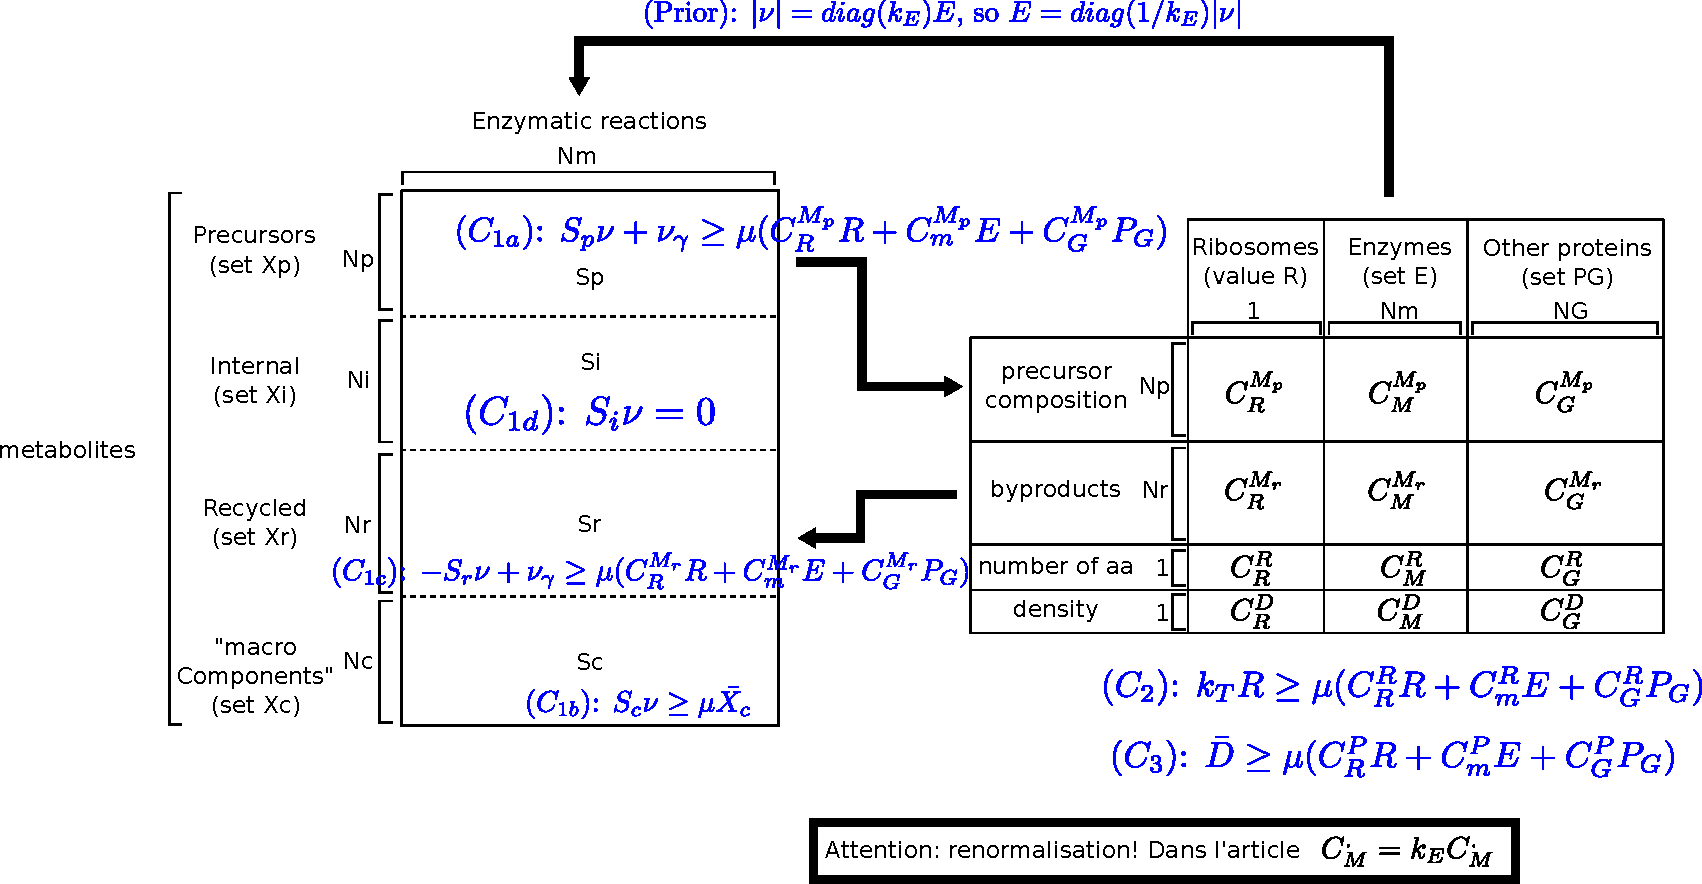
\includegraphics[width=\linewidth]{RBA}
  \caption{Schéma de fonctionnement des RBA.}
  \label{fig:rba}
\end{figure}

\paragraph{Formulation mathématique}

\paragraph{Interprétations mathématiques}

\paragraph{Applications}
\citet{goelzer_cell_2011} applique les RBA à la croissance chez \textit{B. subtilis}. Les cellules croissent dans un milieu qui varie de riche à pauvre. Plus le milieu est riche, plus les bactéries croissent rapidement. Le premier résultat positif est l'augmentation de la part de ribosome et la diminution de la part de protéines métaboliques dans le pool total des protéines. Les auteurs montrent mathématiquement que les RBA permettent de désactiver complètement un pathway à cause de la quantité de protéines nécessaires à maintenir des pathways alternatifs. Quand un a.a. est ajouté au milieu, on observe que sa synthèse \textit{de novo} cesse complètement (ou presque).

La solution des RBA fournit un jeu de régulations qui permettrait d'obtenir un taux de croissance optimal. On peut s'attendre à ce que ces régulations soient effectivement implémentées. D'après \citet{goelzer_cell_2011}, on a un assez bon accord entre prédictions et données. Un exemple avec un switch sur des transporteures à basse et haute affinités est donné pour fournir une illustration simple du phénomène.

Une analyse un peu différente est présentée dans \citet{goelzer_quantitative_2015}. Le but est d'estimer les répartitions globales des ressources chez \textit{B. subtilis}. Le modèle prend en compte le folding via l'introduction de chaperones (mathématiquement de la même façon que les ribosomes). Grâce à de nombreuses données, les efficacités enzymatiques sont estimées (elles étaient fixées de façon \textit{ad hoc} dans \citet{goelzer_cell_2011}). Cela permet de donner un coût en nombre de protéines aux différents sous-processus de la cellule. Une analyse de sensibilité montre que les paramètres liés à la répartition des protéines (densité, fraction de protéines cytosoliques, etc.). Dans le supplementary material, les auteurs montre que les résultats se recoupent partiellement avec une analyse FBA, mais les FBA échouent à allouer correctement les protéines. Globalement le modèle proposé est beaucoup plus riche que dans l'article précédent. J'ai raté beaucoup de subtilités il faudra que je revienne un peu dessus au fur et à mesure.


\subsection{Description du métabolime}
\citet{varma_metabolic_1993, varma_metabolic_1993-1} décrivent assez précisément le catabolisme de base (avec beaucoup de sources à l'appui). On y trouve la description du pathway glycolitique (récupération du glucose), la voie des pentoses phosphates (production de R5P et E4P), le cycle de Krebs (production d'ATP/GTP, NADH) et ses coréactions (shunt glyoxalytique, réactions anaplérotiques). On trouve également la description des chaînes de transport d'électrons et déshydrogénases (production d'ATP, échanges NADH/NADPH/ATP).

\bibliographystyle{myplainnat}
\bibliography{biblio}

\end{document}
% ----------------------------------------------------------------
